การตรวจจับวัตถุนั้นเป็นกระบวนการที่นิยมใช้ในการวิเคราะห์ผลของวิดีโอ กล่าวคือกระบวนการที่ผู้วิจัยจะต้องทำระบุสิ่งที่สนใจว่า คืออะไร อยู่ที่ตำแหน่งใด 
ซึ่งในปัจจุบันการทำการตรวจจับวัตถุมักนำปัญญาประดิษฐ์มาใช้เนื่องจากมีความแม่นยำ และ ช่วยแบ่งเบาภาระของผู้วิจัยในการระบุสิ่งที่สุดใจภายในเฟรม ซึ่งโครงสร้างโมเดลปัญญาประดิษฐ์ของการตรวจจับวัตถุที่ผู้วิจัยสนใจมีดังนี้

\subsubsection*{YOLO}
\begin{figure}[!ht]
    \centering
    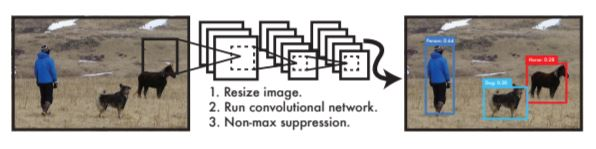
\includegraphics[width=0.7\textwidth]{chapter2/images/yolo.jpg}
    \caption{กระบวนการทำงานของโครงสร้างโมเดลปัญญาประดิษฐ์ของ YOLO}
    \label{fig:yolo}
\end{figure}

โครงสร้างโมเดลปัญญาประดิษฐ์ของ YOLO เป็นโครงสร้างที่มีความเร็วมาก มีความเร็วในการประมวลผลถึง 45 เฟรมต่อวิ ทำให้สามารถประมวลผลแบบเรียลไทม์ได้ นอกจากนั้นยังมีความแม่นยำ mAP มากกว่าโมเดลสำหรับตรวจจับวัตถุอื่นๆถึง 2 เท่า ซึ่งเหตุผลที่โครงสร้างโมเดลปัญญาประดิษฐ์ของ YOLO เร็วกว่าโมเดลปัญญาประดิษฐ์ตัวอื่นๆ เนื่องจาก มีแนวคิดที่ต่างออกไป คือ สำหรับการตรวจจับวัตถุในวิธีการก่อนหน้าจะใช้วิธีทำนายกรอบสี่เหลี่ยมก่อน แล้วจึงค่อยนำกรอบสี่เหลี่ยมไปทำนายว่าเป็นหมวดหมู่อะไร ซึ่ง YOLO มีวิธีการที่ต่างออกไป คือ ทำนายกรอบสี่เหลี่ยมและทำนายว่ากรอบสี่เหลี่ยมนั้นเป็นหมวดหมู่อะไรพร้อมกัน โดยใช้โครงข่ายประสาทแบบคอนโวลูชั่น ด้วยแนวคิดนี้จึงเป็นที่มาของชื่อ YOLO หรือ you only look once การมองแค่เพียงครั้งเดียว ซึ่งโครงสร้างโมเดลปัญญาประดิษฐ์ของ YOLO ที่ถูกใช้ในงานวิจัยนี้ประกอบไปด้วย 1) YOLOv3-tiny 2)YOLOv3 3) YOLOv3-spp	ซึ่งทั้ง 3 โครงสร้างจะมีความแตกต่างของโครงสร้างดังนี้
\begin{enumerate}
	\setlength\itemsep{-0.25em}
	\item YOLOv3-tiny ใช้ Max-Pooling layers ในขั้นตอนของการลดจำนวนข้อมูลตัวอย่าง
	\item YOLOv3 ใช้ Convolutional layers ในขั้นตอนของการลดจำนวนข้อมูลตัวอย่าง
	\item YOLOv3-spp ใช้ Convolutional layers+ฟีเจอร์ที่ดีที่สุดของ Max-Pooling layers ในขั้นตอนของการลดจำนวนข้อมูลตัวอย่าง
\end{enumerate}
%ข้อมูลผลการทำงานของโมเดลปัญญาประดิษฐ์สำหรับการทำการตรวจจับภาพบุคคล อ้างอิงข้อมูลจากเว็บไซต์ของ YOLO
%\begin{table}[!ht]
%	\begin{tabular}{|c|c|c|}
%		\hline
%		{}&{ความเร็วต่อรูปภาพ (มิลลิวินาที)}&{ความแม่นยำ (0.5 IoU mAP)}			\\
%		\hline
%		SSD Mobilenet v1 ppn	 		& 26				& 20														\\
%		YOLO-v3 320				& 22				& 51.5				\\	
%		YOLO-v3 tiny				& 4.5				& 33.1				\\
%		YOLO-v3 spp				& 50				& 60.6				\\	
%		Faster RCNN inceptrion v2		& 58				& 28		\\
%	\hline
%	\end{tabular}
%	\caption{ข้อมูลผลการทำงานของโมเดลปัญญาประดิษฐ์สำหรับการทำการตรวจจับภาพบุคคล อ้างอิงข้อมูลจากเว็บไซต์ของ YOLO}
%\end{table}

